\section{The known-world packets, re-read under the battery}
\label{sec:known-world}

The objective known-world lane predates the battery of Section~\ref{sec:falsifiability}. This section preserves its registered outcomes exactly as executed and then states what they are worth under the battery's findings. Nothing here is softened; the numbers stand, and their reading changes.

\subsection{The four-family confirmatory packet: registered outcome}

The lane was designed so that the correct transfer decision is obtained by executing a family-specific target-world verifier rather than by an annotator or by the generator's perturbation identity. Four heterogeneous exact-verifier families were frozen before confirmatory outcome access: mapped directed-flow feasibility, Horn-style logical entailment, dimensional/unit transformations and finite deterministic state-transition systems. The first development instrument failed the preregistered coordinate-ablated-twin circularity attack and was preserved as negative history rather than promoted. A redesigned development instrument passed the registered checks; its paired variance gave a required decidable sample of 431 for the registered $0.05$ MDE, and seed \texttt{2026081202} with $n=576$ total cases (256 verifier-licensed, 256 verifier-rejected, 64 \texttt{CANNOT\_CHECK}) was frozen and merged publicly before execution.

The registered outcome: a lexical/Jaccard control sat at chance on the 512 decidable cases (accuracy $0.496$). A derived-effect (``mechanism-only'') rule reached exact three-way accuracy $0.875$ and accepted every valid transfer, but licensed $25\%$ of verifier-invalid transfers; a relation/invariant-only rule reached $0.819$ with $37.5\%$ invalid false-accepts at full valid retention. The full applicability contract matched all 576 verifier decisions---every valid transfer retained, no invalid transfer licensed, every verifier-unknown case abstained. The preregistered primary statistic, paired binary-Brier reduction of the full contract against the mechanism-only control, was $0.120$ with item-bootstrap 95\% interval $[0.0938,0.1481]$; the four-family sign test is $p=0.125$, which is why a six-family extension was frozen as a separate coordinate. That extension was later executed, passed, and audited---Section~\ref{sec:six-family}.

\subsection{What the battery leaves standing}

The battery findings on the six-family sibling packet apply to this lane's architecture, and the manuscript must say so plainly rather than by understatement. Candidate inputs in the objective lane expose machine-readable target-world facts from which the deterministic coordinates are computed; probe~G, executed on the six-family packet built from the same architecture, shows the stronger fact that the benchmark surface carries \emph{zero} extraction signal---not merely insufficient signal---because no decision arm reads the text at all. The full arm implements the same coordinate algebra the verifier executes, so its exact agreement is a consistency property of the construction, and the control-arm deficits quantify which strata the generator contains (probe~F: in the six-family packet, two thirds of the headline gain came from strata the control could not see by design).

What stands, therefore, is a \emph{specification demonstration}: the contract's six coordinates are individually enforceable, jointly sufficient on the registered families, and the deterministic pipeline---generation, freezing, hashing, execution, paired inference---runs to completion and reproduces its registered outputs byte-for-byte. The reading ``checking a subset of the six independent conditions misses violations of the others'' is arithmetic once probe~G is known, and we report it as arithmetic, not as an empirical transfer finding. Per the battery's probe-C corollary, no false-accept figure above is reported without its paired retention figure. The lane establishes no claim that a system recovers applicability coordinates from unstructured input, no model-level claim, and no natural-domain claim.

\subsection{A demoted external-model comparator}
\label{sec:llm-comparator}

One measured external-model result is retained, at deliberately demoted authority. An independently frozen comparator drove one fixed frontier model through the fail-closed applicability contract on $n\approx504$ fresh exact-verifier tasks (seed \texttt{20260812}; design, primary metric, hypothesis direction and stopping rule frozen before any output was scored), against a plain \textsc{Direct} judgement and a compute-matched \textsc{Free-CoT} control, with the same three-way label space in every arm.

\begin{figure}[t]
\centering
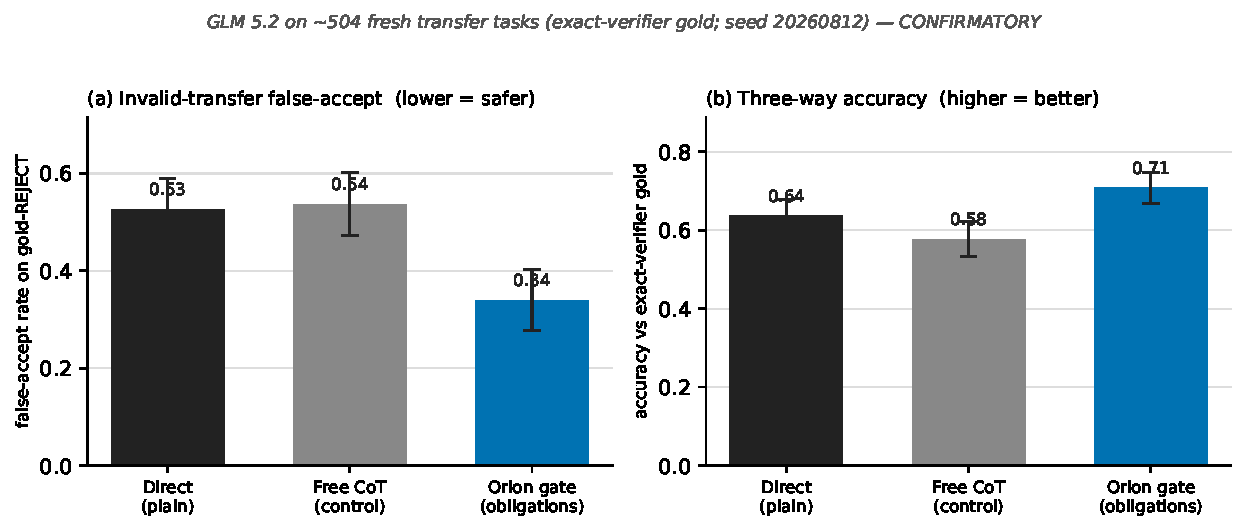
\includegraphics[width=\textwidth]{figures/llm_comparator.pdf}
\caption{Demoted external-model applicability-gate comparator (one fixed frontier model; $n\approx504$ fresh exact-verifier tasks; bootstrap $95\%$ CIs, 20{,}000 resamples). \textbf{(a)}~Driving the model through the fail-closed applicability gate cuts the invalid-transfer false-accept rate from $0.527\,[0.460,0.589]$ (Direct) to $0.339\,[0.277,0.402]$ (gate); the compute-matched Free-CoT control ($0.536\,[0.473,0.603]$) is statistically indistinguishable from Direct. \textbf{(b)}~Three-way accuracy against exact-verifier gold rises in step ($0.637$ Direct $\to0.708$ gate), while the compute-matched control falls to $0.577$: the extra reasoning tokens cost accuracy where the obligation structure gains it. The benchmark surface was subsequently shown to carry no extraction requirement (Section~\ref{sec:six-family}, probe G), so this measures compliance with the obligation structure over structured inputs---a scaffold effect---not prose reading or model reasoning quality; on the hardest semantic near-miss decoys the gate is \emph{worse} than Direct ($0.357$ against $0.268$ false-accept) and exactly ties the \textsc{Free-CoT} control it otherwise dominates ($0.357$), a real and reported weakness.}
\label{fig:llm-comparator}
\end{figure}

Figure~\ref{fig:llm-comparator} shows the obligation scaffold roughly halving the odds of licensing a verifier-invalid transfer while the compute-matched control moves nothing: the reduction is attributable to the obligation \emph{structure}, not to additional reasoning tokens. Three demotions bound this result. It is one model (\texttt{glm-5.2}), one seed and one family-set. It measures a structured-inference scaffold, not a smarter model, and on the hardest semantic near-misses it does not merely fail to help: it raises the false-accept rate above \textsc{Direct} ($0.357$ against $0.268$) and lands exactly on the \textsc{Free-CoT} control ($0.357$). That coincidence is the sharper reading. The result's whole force is that the reduction is attributable to obligation structure rather than to reasoning tokens, evidenced by \textsc{Free-CoT} moving the aggregate false-accept rate not at all; on the decoy slice the scaffold and the token control are indistinguishable, so whatever separates them elsewhere is absent exactly where the discrimination is hardest. The gate's aggregate advantage is therefore scoped to invalid transfers that are not semantic near-misses. And---decisive after the battery---the underlying benchmark's coordinates travel in pre-parsed form, so the comparator measures whether the model \emph{applies} the named obligations to structured facts, not whether it can recover them. A cross-model, cross-seed replication on a battery-compliant benchmark is the named next coordinate before any external-model claim.
